\documentclass{mpaper}
\usepackage{amsthm}
\newtheorem{definition}{Definition}[section]

\begin{document}

\title{Counting Monochromatic Components in Adversarial Graph Burning}
\author{Lewis Dyer}
\matricnum{2299195}

\maketitle

\begin{abstract}
According to Simon Peyton Jones, an abstract should address
four key questions. First, what is the problem that this
paper tackles? Second, why is this an interesting problem?
Third, what is the solution this paper proposes?
Finally, why is the proposed solution a good one?
\end{abstract}

\section{Introduction}

This paper outlines the standard template for an MSci submission.
In earlier years, MSci students at the School of Computing
Science\footnote{\url{http://www.dcs.gla.ac.uk}},
University of Glasgow, were expected to produce a full-length
dissertation. Now, the requirement is for MSci students to
write a paper of up to 14 pages in length, using the supplied
\texttt{mpaper} \LaTeX style file.

The precise structure of an MSci paper is not mandated, but it should
probably cover in detail the following aspects of the project.
\begin{enumerate}
\item General description of the problem, motivation, relevance
\item Background information, possibly including a literature survey
\item Description of approach taken to solve the problem, including
  high-level design and lower-level implementation details as appropriate
\item Evaluation, qualitative or quantitative as appropriate
\item Conclusion, including scope for future work
\end{enumerate}

\section{Background}

This \LaTeX template is based on the ACM \texttt{sig-alternate} class.
The layout is two-column text. Generally figures and tables only
extend to one column width, e.g.\ Table \ref{tab-eg},
but it is possible to make them
stretch over both columns using the \texttt{figure*} and
\texttt{table*} environments. For an example, see Figure \ref{fig-eg}.

\begin{table}
\begin{tabular}{l||c||p{2cm}}
\emph{Operating System} & \emph{Version} & \emph{Verdict} \\ \hline \hline
Ubuntu & 12.04 & Everyone's favourite Linux, unless you grew up with
RedHat \\ \hline
Slackware & xxx & Pseudo-hacker's Linux, how often do you recompile
your kernel? \\ \hline
Mac OS & 10.7 & For people with more money than sense \\ \hline
\end{tabular}
\caption{\label{tab-eg}Single column table of figures}
\end{table}

\begin{figure*}
\begin{center}
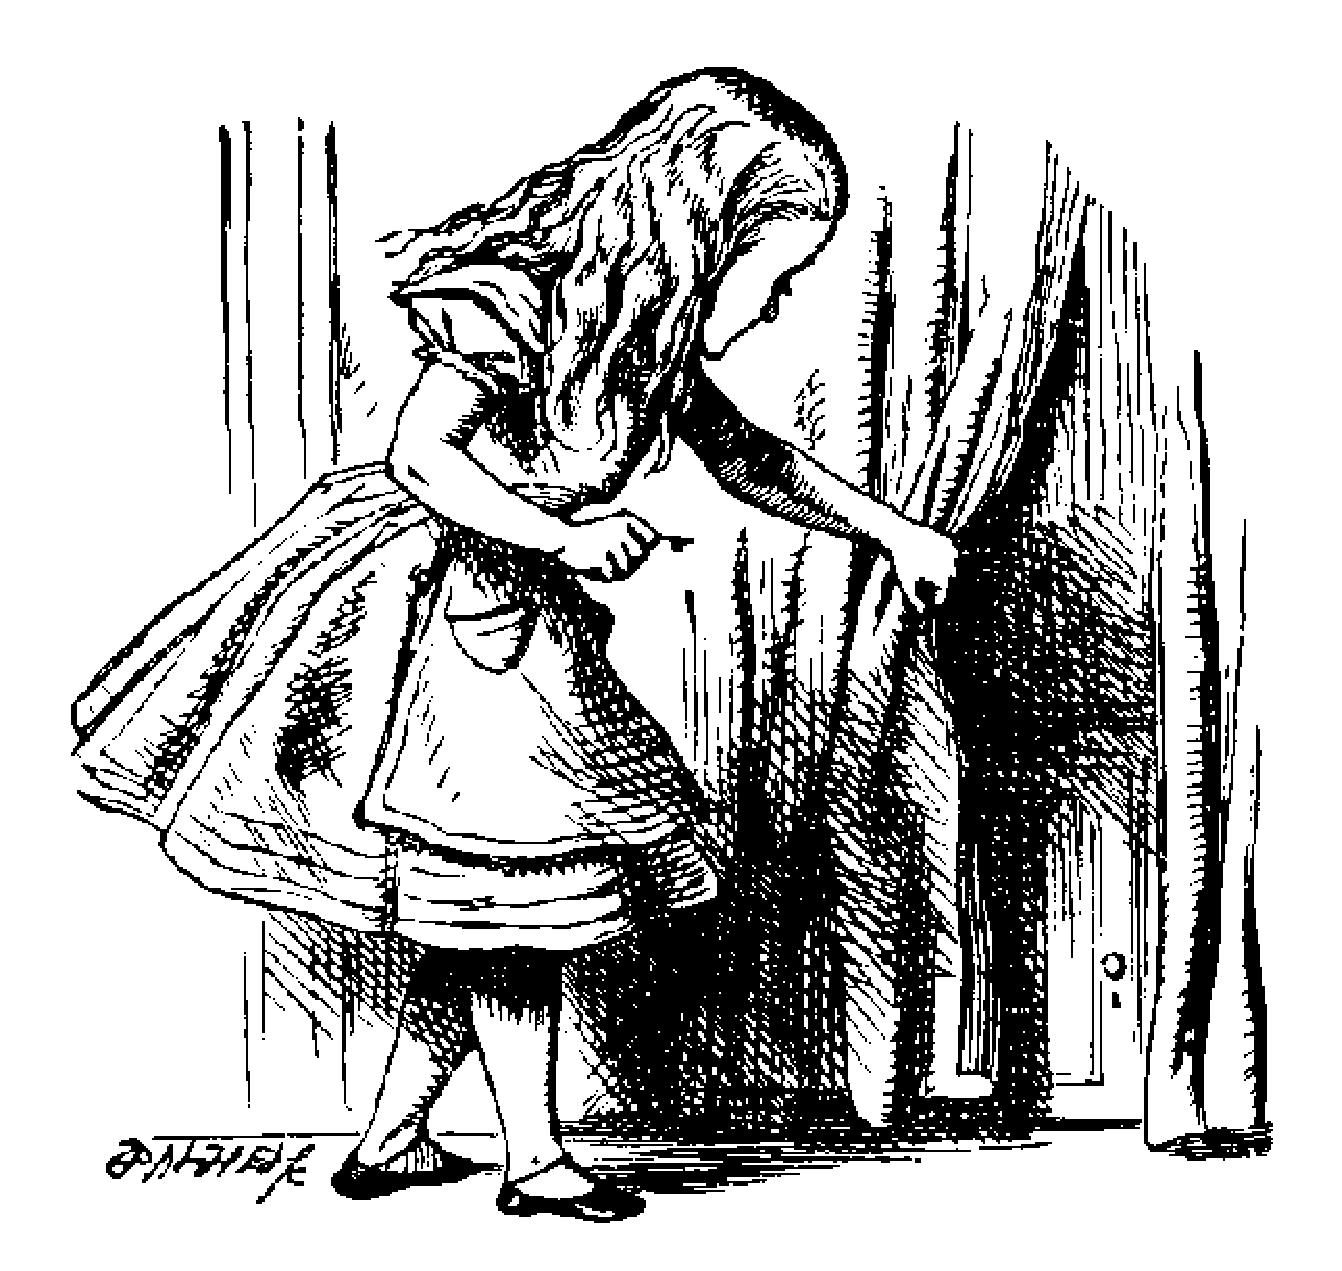
\includegraphics[scale=0.3]{alice.pdf}
\end{center}
\caption{\label{fig-eg}An example figure stretching over two columns}
\end{figure*}

\section{The WizWoz System}

Again, Simon Peyton Jones has a lovely description of how to write a
paper on his
website\footnote{\url{http://research.microsoft.com/en-us/um/people/simonpj/papers/giving-a-talk/giving-a-talk.htm}}.
Personally, I put URLs in footnotes and \emph{bona fide} references
in the bibliography. For instance, Turing \cite{turing37computable}
and Knuth \cite{knuth68art} would not be out of place in list of
references.
How many references? Hard to say. Five is not enough, 50 is pushing
it.


\section{Adversarial Graph Burning}
% define AGB formally (not sure if defining regular graph burning is needed formally?)

\subsection{Defining Adversarial Graph Burning}

First, we formalise the process of Adversarial Graph Burning on a graph $G$. Throughout, we presume that $G$ is a finite, simple, undirected graph.

\begin{definition}
\label{def/AGB}

Adversarial Graph Burning (or AGB for short) is a discrete-time graph process for two players (and by convention, player 1 and 2 are red and blue, respectively). Each vertex is assigned one of 4 colours:

\begin{enumerate}
  \item \emph{White} vertices have not been burned by either player yet.
  \item \emph{Red} vertices have been burned by player 1.
  \item \emph{Blue} vertices have been burned by player 2.
  \item \emph{Green} vertices have been burned by \emph{both} players.
\end{enumerate}

At time $t=0$, all vertices are white. At each time $t > 0$, each player simultaneously chooses one white vertex to burn.

\end{definition}

\subsection{Burning Sequences}

\subsection{Bounding the length of burning sequences}

\section{Counting Monochromatic Components}

\subsection{Monochromatic components on paths}

\subsection{Caterpillar graphs}

\subsection{Monochromatic components on caterpillar graphs}


{\bf Acknowledgments.}
Firstly, I would like to thank my supervisors - Jessica Enright, William Pettersson and John Sylvester - for their continual guidance and support throughout the project. I wouldd also like to thank my parents, for always caring for me, and supporting my goals when I thought they could never be attained. And, last but not least, I would like to thank my girlfriend Jodie, for her never-ending love and kindness.

\bibliographystyle{abbrv}
\bibliography{example}


\end{document}